\documentclass{article}
\usepackage[left=3cm,right=3cm,top=2.5cm,bottom=2cm]{geometry} % page settings
\usepackage{amsmath} % provides many mathematical environments & tools
\usepackage{amssymb}
\usepackage{amsfonts}
\usepackage[spanish]{babel}

\usepackage{multirow}

\usepackage{algorithm}
\usepackage{algpseudocode}
\usepackage{pifont}

\usepackage[utf8]{inputenc}
\setlength{\parindent}{0mm}

\usepackage[parfill]{parskip}

% Para el código
\usepackage{listings}
\usepackage{xcolor}
\definecolor{gray}{rgb}{0.5,0.5,0.5}
\newcommand{\n}[1]{{\color{gray}#1}}
\lstset{numbers=left,numberstyle=\small\color{gray}}

% Entorno para estilo de ejercicios
\setlength{\parindent}{0pt}

\usepackage{color}   %May be necessary if you want to color links
\usepackage{hyperref}
\hypersetup{
    colorlinks=true, %set true if you want colored links
    linktoc=all,     %set to all if you want both sections and subsections linked
    linkcolor=blue,  %choose some color if you want links to stand out
}

\usepackage{graphicx}
\usepackage{subfig}

\usepackage{listings,textcomp}
\lstset{
  breakatwhitespace,
  language=c++,
  columns=fullflexible,
  keepspaces,
  breaklines,
  tabsize=2, 
  showstringspaces=false,
  extendedchars=true,
  basicstyle=\fontfamily{pcr}\selectfont\scriptsize,
  keywordstyle=\color{orange},
  upquote=true,
  literate={-}{-}1
}

\lstset{numbers=left,xleftmargin=3.5em,framexleftmargin=1em}

\title{Aplicación del algoritmo Divide y Vencerás \\[5mm]
  \Large Algorítmica\\
  \normalsize Doble Grado en Ingeniería Informática y Matemáticas\\[5cm]
}
\author{Yábir García Benchakhtir \\ yabirgb@correo.ugr.es \\[10cm]}

\date{\today}

\begin{document}

\maketitle

\section{Descripción del problema}

Para poner en práctica este algoritmo se nos presenta inicialmente un
vector de números comprendido en un intervalo $[-M, M]$ de modo que se
escojen numeros de manera aleatoria de ese intervalo y se crea un
vector de un tamaño $N$. Posteriormente se aplica el algoritmo sort
que incorporla la libería \textit{algorithm} de \textit{C++}.

Bajo esta hipótesis tenemos que crear un algoritmo de manera que
encontremos, si existe, un elemento del vector(\textit{v}) tal que
$v[i] = i$.

\section{Algoritmo desarrollado}

El problema se basa en realizar la busqueda de un elemento que
satisfaga una determinada condición y lo queremos resolver aplicando
la técnica Divide y Vencerás. Este problema se parece bastante al
problema de la busqueda binaria luego es razonable plantearse si
nuestro algoritmo se puede basar en este.

\begin{lstlisting}
int inpos(vector<int> &v){
  int min = 0;
  int max = v.size();
  int mid;

  while (min <= max){
    mid = (max+min)/2;
    
    if (v[mid] == mid)
      return mid;
    else if(v[mid] < mid)
      min = mid + 1;
    else if(v[mid] > mid)
      max = mid-1; 
  }

  return -1;
}
\end{lstlisting}

En este caso lo que estamos aplicando es el mismo algoritmo que en la
busqueda binaria, pero en este caso en lugar de comprobar si la
posición central es un número fijo, estamos buscando un número que
depende de la posición que estamos comprobando.

Para comparar los resultados de este algoritmo desarrollamos un
algoritmo que simplemente itera sobre todas las posiciones buscando si
se satisface la condición que queremos.

\begin{lstlisting}
int inposOdd(vector<int> v){

  int i;

  for(i = 0; i < v.size(); i++)
    if(v[i] == i)
      return i;

  return -1;
}
\end{lstlisting}

Para estudiar la eficiencia del primer algoritmos tenemos que observar que lo que estamos haciendo es o devolver un valor o llamar a la misma función cambiando los argumentos. En cada iteración del algoritmo trabajamos únicamente con la mitad del vector, de este modo tenemos que:

\[
  T(n) = T(n/2) + a
\]

y la complejidad de este algoritmo es $O(log(n))$

En el caso del segundo algoritmo la complejidad es $O(n)$

\section{Mediciones realizadas}

\subsection{Metodología para el estudio de los algoritmos}

Para estudiar el grado de eficiencia de ambos algoritmos se ha usado
un archivo de código \textit{C++} donde se han añadido ambos
algoritmos como funciones independientes y se ha generado un único
vector ordenado de manera que se han aplicado ambos algoritmos sobre
el mismo vector.

Para medir el tiempo de ejecución de ambos algoritmos se ha utilizado
la librería \textit{ctime} y la función \textit{clock}.

En cada tamaño marcado se han realizado dos mediciones con vectores
distintos y se han recopilado los tiempos de ejecución. Las mediciones
se han tomado de 1 a 1000000 incrementando el tamaño de 10000 en
10000 números.

\subsection{Condiciones de las mediciones}

El programa descrito se ha compilado usando \textit{g++} en su versión
\textit{g++ (Ubuntu 5.4.0-6ubuntu1~16.04.9) 5.4.0 20160609} en una máquina con las siguientes especificaciones:


\begin{itemize}
\item CPU: Intel Pentium G3258 (2) @ 3.200GHz
\item Memoria RAM: 7876MiB
\item Kernel: 4.13.0-36-generic
\item OS: Linux Mint 18.3 Sylvia x86\_64
\end{itemize}

\subsection{Resultado de las mediciones}

Debido al gran tamaño de las mediciones se adjuntan estas en el
documento llamado \textit{mediciones.out}. He representado los datos
en la siguiente gráfica.

\begin{figure}[H]
  \centering   
      \subfloat{%
        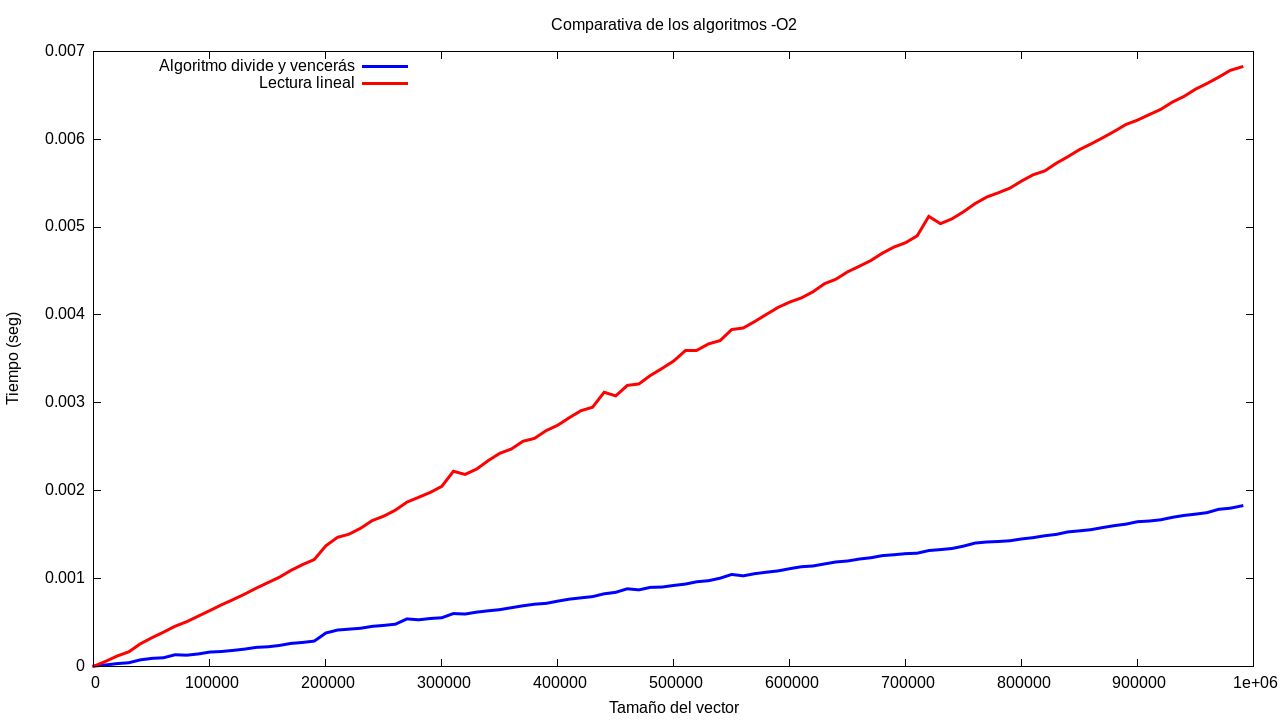
\includegraphics[clip,width=1\columnwidth]{../plots/copia_4.png}%
      }

\caption{Comaparación de los dos algoritmos}
\end{figure}

Analizando la eficiencia híbrida del algoritmo planteado le hacemos
regresión mediante una función del tipo $f(x) = b*log(x+c)+a$ y tras
1326 iteraciones gnuplot nos da como resultado la siguiente regresión.

\begin{figure}[H]
  \centering   
      \subfloat{%
        \includegraphics[clip,width=1\columnwidth]{../plots/hibrida2.png}%
      }

\caption{Eficiencia híbrida ($log(n)$}
\end{figure}

\begin{verbatim}
Final set of parameters            Asymptotic Standard Error
=======================            ==========================

a               = -0.189463        +/- 0.02642      (13.95%)
b               = 0.0121242        +/- 0.001582     (13.05%)
c               = 6.10404e+06      +/- 8.595e+05    (14.08%)
\end{verbatim}

Donde vemos que el ajuste es muy buen aunque si hacemos un ajuste lineal observamos: 

\begin{figure}[H]
  \centering   
      \subfloat{%
        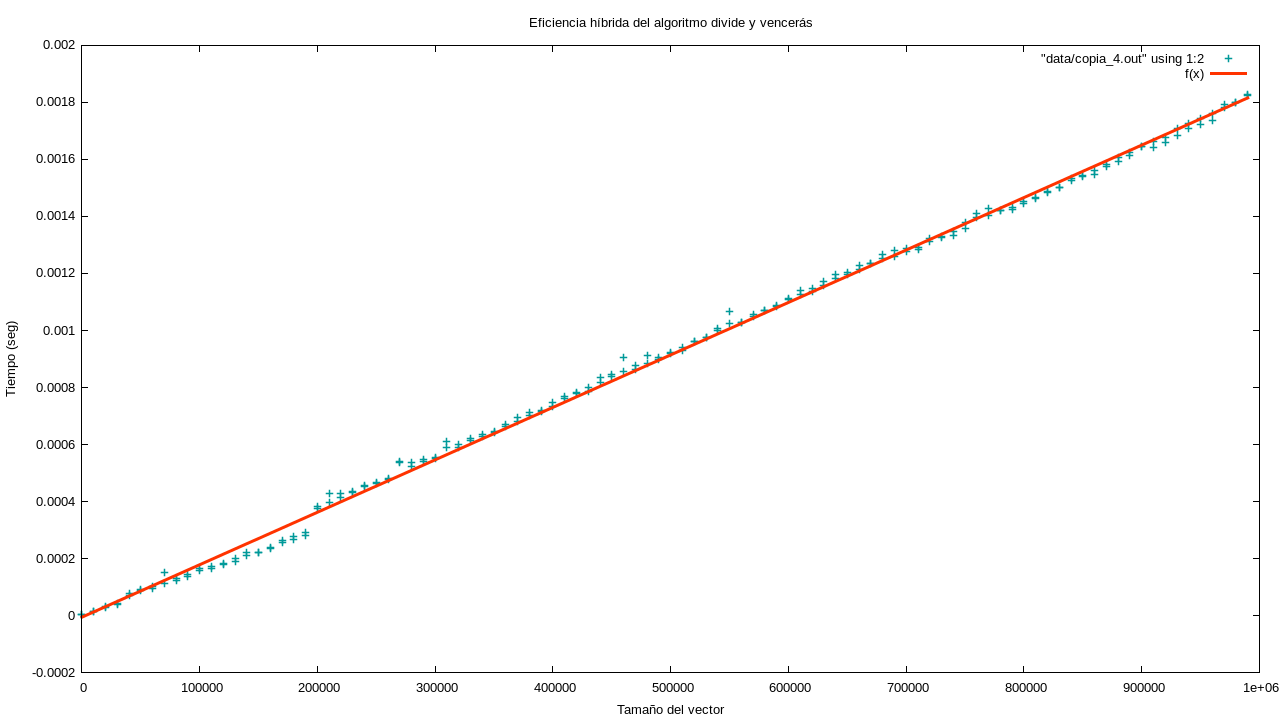
\includegraphics[clip,width=1\columnwidth]{../plots/hibrida_lineal.png}%
      }

\caption{Eficiencia híbrid $mx+n$}
\end{figure}

\begin{verbatim}
Final set of parameters            Asymptotic Standard Error
=======================            ==========================

a               = -5.18976e-06     +/- 2.963e-06    (57.1%)
b               = 1.83948e-09      +/- 5.171e-12    (0.2811%)

\end{verbatim}

Que nos indica que aun siendo bueno el ajuste logarítmico tiende a
comportarse como una recta para valores pequeños.

\section{Mejora de nuestro algoritmo}

El algoritmo implementado anteriormente no funciona cuando en el
vector encontramos elementos repetidos ya que esto hace que la
dependencia entre el orden y la posición al comparar no sea tal. Para
resolverlo se propone la siguiente implementación de un algoritmo
Divide y Vencerás:

\begin{lstlisting}
int conRepetidos(vector<int> &v, int top, int bot){

  if (bot > top)
    return -1;

  int mid = (top+bot)/2;
  int midv = v[mid];

  if (midv == mid)
    return mid;

  int lefti = min(mid-1, midv);
  int left  = conRepetidos(v, lefti, bot);

  if (left != -1)
    return left;

  int righti = max(mid+1, midv);
  int right = conRepetidos(v, bot, top);

  return right;
      
}
\end{lstlisting}

En esta implementación estamos aplicando un desarrollo semajante al
anterior pero en esta ocasión tenemos en cuenta un entorno del punto
que analizamos.

Como demuestra el siguiente gráfico

\begin{figure}[H]
  \centering   
      \subfloat{%
        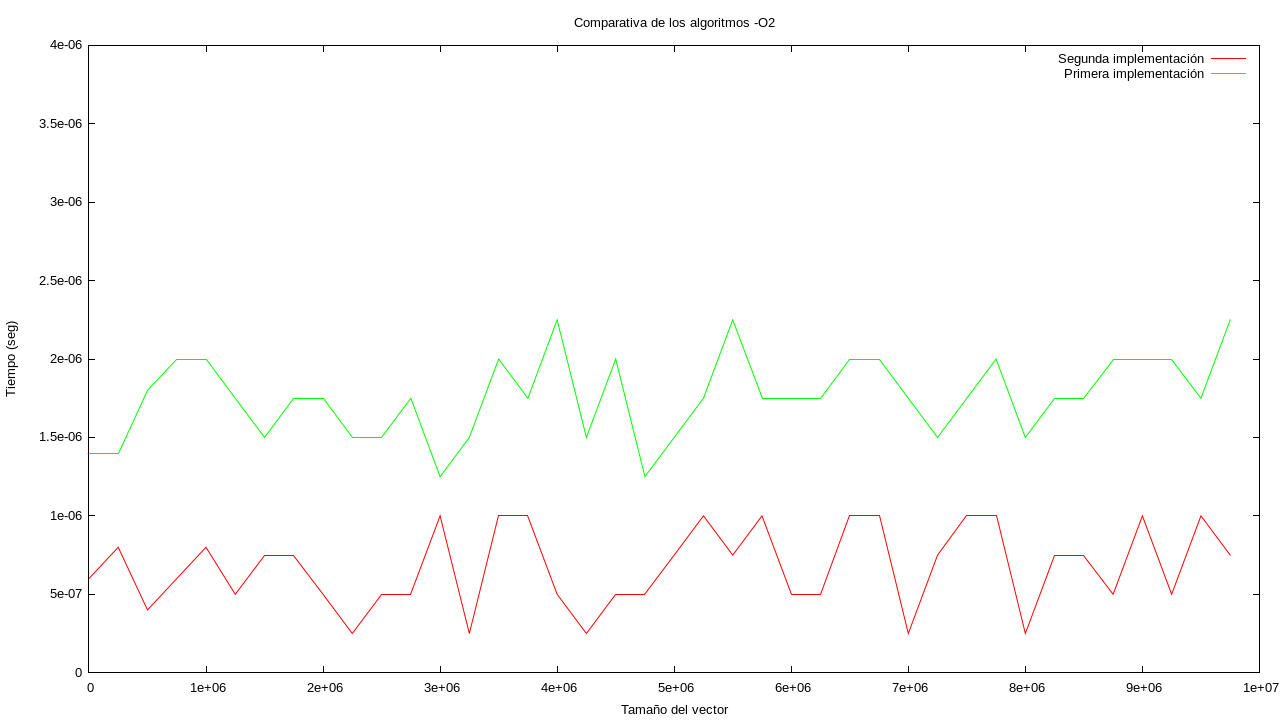
\includegraphics[clip,width=1\columnwidth]{../plots/segundoDyV.png}%
      }

\caption{Comparación de ambos algoritmos DyV}
\end{figure}
la eficiencia del nuevo algoritmos es mayor además de ser más general
que el anterior.

Un análisis teórico del algoritmo anterior nos permite ver que la
eficiencia es también logarítmica y al ver la comparativa de tiempos
entre ambos podemos afirmar esto ya que la linea de tiempos se
mantiene paralela a la del primer algoritmo.

\end{document}
